% !TEX root = ../discriminative_filtering.tex

\section{Preface}
The remainder of this chapter has been submitted to the Journal Neural Computation as an article entitled ``Robust closed-loop control of a cursor in a person with tetraplegia using Gaussian process regression.'' David Brandman had the idea to explore robustness, conducted the online experiments with human volunteers, and wrote much of the paper.  The kernel selection for the Gaussian process was worked out by myself and Prof. Harrison.  We are grateful to our co-authors Prof. Hochberg, J. Kelemen, and B. Franco at BrainGate for making this investigation possible.

\section{Abstract}
Intracortical Brain computer interfaces can enable individuals with paralysis to control external devices. Decoding quality has been previously shown to degrade with signal nonstationarities, including changes to the neural tuning profiles, baseline shifts in firing rates, and non-physiological noise. While progress has been made towards providing long-term user control via decoder recalibration, relatively little work has been dedicated towards making the decoder itself more resilient to signal nonstationarities. Here, we describe how principled kernel selection with Gaussian process regression can be used within a Bayesian filtering framework to mitigate the effects of  a commonly-encountered type of nonstationarity (large changes in a single neuron).  Given a supervised training set of (neural,intention)-pairs, we use a Gaussian process regression with a specialized kernel (a multiple kernel) to estimate intention(t)|neural(t).  This multiple kernel sums over each individual neural dimension, allowing the kernel to effectively ignore large differences in neural vectors that occur only in a single neuron. The summed kernel is used for real-time predictions of the posterior mean and variance of intention(t)|neural(t) using a Gaussian process regression framework. The Gaussian process predictions are then filtered using the discriminative Kalman filter to produce an estimate for intention(t)|neural(1:t). We refer to the multiple kernel approach within the DKF framework as the MK-DKF. We found that the MK-DKF decoder was more resilient to non-nonstationarities frequently encountered in-real world settings, yet provided similar performance to the currently used Kalman decoder. These results demonstrate a method by which neural decoding can be made more resistant to nonstationarities.

\section{Introduction}

Brain Computer Interfaces (BCIs) use neural information recorded from the brain for the voluntary control of external devices \cite{Wolpaw2002, Hochberg2006, Schwartz2006, Lebedev2006, Fetz2007, Chestek2009, Carmena2013}. At the heart of BCI systems is the decoder: the algorithm that maps neural information to generate a signal used to control external devices. Modern intracortical BCI decoders used by people with paralysis infer a relationship between neural features (e.g. neuronal firing rates) and the motor intentions from training data. Hence, high quality control of an external effector, such as a computer cursor, is predicated on appropriate selection of a decoding algorithm. 

Decoder selection for intracortical BCI (iBCI) systems traditionally has been based on extensive study of cortical physiology. In what are now classic experiments, non-human primates (NHPs) were taught to move a planar manipulandum to one of eight different directions \cite{Georgopoulos1982}. The firing rate as a direction of arm movement was parsimoniously modeled as a sinusoidal curve. For each neuron, the vector corresponding to the maximum firing rate (i.e. the phase offset of a cosine-function with a period of 360 degrees) is often referred to as the neuron's ``preferred direction''. The population vector algorithm scales the preferred directions of the recorded neurons by their recorded firing rate; the sum is the decoded vector of the intended direction of neural control \cite{Taylor2002, Jarosiewicz2008, Velliste2008}. Given sufficient diversity in preferred directions, the problem reduces to linear regression: decoding involves learning the least-squares solution to the surface mapping firing rates to kinematic variables \cite{Kass2005}. Alternative decoding approaches include modeling the probability of observing a neural spike as a draw from from a time-varying poisson process \cite{Truccolo2008, Brown2002, Ba2014, Shanechi2017}; using support-vector regression \cite{Shpigelman2008} or neural networks \cite{Sussillo2016a}.

\index{neural filtering!nonstationarities} 
An ongoing area of research in iBCI systems is to ensure robust control for the user. Degradation in neural control is often attributed to nonstationarities in the recorded signals. With linear models, changes to the baseline firing rate, preferred direction, or depth of modulation result in degradation in decoding performance \cite{Sussillo2015, Jarosiewicz2015, Perge2013}. The most common approach to addressing this mismatch involves recalibrating the decoder's parameters by incorporating more recent neural data. This has been described using batch-based updates during user-defined breaks \cite{Jarosiewicz2015, Bacher2015, Gilja2015}, batch-based updates during ongoing use \cite{Orsborn2014, Shpigelman2008}, and continuous updating during ongoing use \cite{Shanechi2014, Shanechi2016, Dangi2011}. Ongoing decoder recalibration traditionally requires information regarding the cursor's current location and a known target; alternatively, retrospective target inference has been described as a way to label neural data with the BCI users' intended movement directions based on selections during self-directed on-screen keyboard use \cite{Jarosiewicz2015}.  

While attempts to mitigate nonstationarities have largely focused on recalibration, few efforts have aimed to make the decoder inherently more resilient to nonstationarities. To our knowledge, the most extensive study of examining decoder robustness investigated the use of deep neural networks trained from large amounts of offline data \cite{Sussillo2016a}. While effective for decoding, this method requires tremendous computational data and resources, and required the decoder to be specifically ``trained'' to handle nonstationarities using extensive regularization. 

\index{Discriminative Kalman Filter!use with a robust model}
Here, we demonstrate a new decoding algorithm that is more resilient to signal nonstationarities than the currently used linear decoding models. Our approach builds on the previously well-established linear state-space dynamical model for neural decoding. Building upon prior work \cite{Brandman2018}, the key innovation is making a nonlinear decoder robust to noise through kernel selection and data sparsification. In this report, we have modified the kernel used for the Gaussian process decoder such that it is more resilient to nonstationarities. We refer to this new method as the MK-DKF method.

\section{Mathematical Methods}

We have previously described closed-loop decoding using Gaussian process regression (GP) in detail \cite{Brandman2018}. Briefly: a collection of neural features, $\xi_i$, and inferred velocity vectors, $\zeta_i$, for $1 <= i <= n$, are collected during calibration. To perform closed-loop neural decoding at time step $t$, new neural features, $x_t$, are compared to $\xi_i$ according to a similarity metric (e.g. radial basis function). The $n$ similarities are then used to scale the corresponding $\zeta_i$ labels.  The current unfiltered estimate, $f(x_t)$ for the expected value of $Z_t|X_t$ is given by the sum of the scaled $\zeta_i$ values.  Filtering then produces an estimate $\mu_t$ for the mean of $Z_t|X_{1:t}$; this value $\mu_t$ is returned by the decoder.

Our previous approach to GP decoding used the entire high-dimensional neural dataset as the basis for computing the measure of similarity between $x_t$ and $\xi$ \cite{Brandman2018}. In this report, we made two important changes to the decoder to increase its robustness to signal nonstationarities. 

First, we adopted a kernel that calculated the similarity between two neural vectors as the arithmetic average over similarities in each neuron, as opposed to the product that was used by the more standard isotropic Gaussian kernel (see Section~\ref{s:kernel_selection}).  This had the effect of limiting the impact any single neuron could have on the calculated similarity between two vectors of neural features. When a nonstationarity occurred in a feature, the decoder ``disregarded'' this feature without compromising decoding quality. 

Second, we sparsified the data by averaging $(\xi, \zeta)$ pairs into octants. This dramatically decreased the computational load for real-time decoding. We found that the observed neural features had noise events with surprising frequency (see Results). Without data sparsification, the training features contained a large number of noisy features which were then used for decoding. Averaging across octants had the effect of mitigating the importance of these noisy features for decoding.  

%We are not entirely sure why sparsifying the data had an impact on noise resilience, but we do believe it's related to addressing the large numbers of noise events in our dataset. More specifically

\subsection{Description of decoding method}

We model the latent state space model with hidden states $Z_1,\dotsc,Z_T \in \RR^d$ representing the intended cursor velocity, and the observed states $X_1,\dotsc,X_T \in \RR^m$ representing the neural features related through the following graphical model:
\[
%\resizebox{\hsize}{!}{}
\begin{CD}
Z_1 @>>> \cdots @>>>  Z_{t-1} @>>> Z_t @>>> \cdots  @>>> Z_T \\
@VVV @.	@VVV @VVV @. @VVV \\
X_1  @. @. X_{t-1} @. X_t @. @. X_T
\end{CD}
\]
In typical use, $d$ is 2 dimensional (e.g kinematic computer cursor control) while $m$ is 40 \cite{Jarosiewicz2013, Jarosiewicz2015, Bacher2015, Brandman2018}.  Each dimension of $X$ corresponds to a neural feature. We are interested in the posterior distribution $p(z_t|x_{1:t})$ of the current hidden state given all observations up to present. Upon specifying the state model $p(z_t|z_{t-1})$ that relates how the hidden state changes over time and the measurement model $p(x_t|z_t)$ that relates the hidden and observed variables, the posterior can be found recursively using the Chapman--Kolmogorov equation
\begin{equation}
\label{e:chapman_kolmogorov}
p(z_t|x_{1:t}) \propto p(x_t|z_t) \int p(z_t|z_{t-1}) \; p(z_{t-1}|x_{1:t-1})\; dz_{t-1},
\end{equation}
where $\propto$ means proportional as a function of $z_t$. The standard Kalman filter is obtained when both the state and measurement models are specified as linear with Gaussian noise \cite{Wu2005, Simeral2011}.  Here, we use a stationary, linear state model with Gaussian noise 
\begin{subequations} \label{e:statemodel}
\begin{align}
 p(z_0) & = \eta_d(z_0;0,S), \\ 
 p(z_t|z_{t-1}) & = \eta_d(z_t;Az_{t-1},\Gamma),
\end{align}
\end{subequations}
where $A,S,\Gamma$ are $d\!\times\!d$, $S$ and $\Gamma$ are proper covariance matrices, $S=ASA^\intercal+\Gamma$, and $\eta_d(z; \mu, \Sigma)$ denotes the $d$-dimensional multivariate normal density with mean $\mu$ and covariance $\Sigma$ evaluated at a point $z$. We approximate the measurement model using Bayes' rule,
\begin{equation}
\label{e:measurement_model}
p(x_t|z_t) 
\propto \frac{p(z_t|x_t)}{p(z_t)}
\approx \frac{\eta_d(z_t; f(x_t), Q)}{\eta_d(z_t; 0, S)},
\end{equation}
where $f:\RR^m \rightarrow \RR^d$ is a nonlinear function learned from training data and $Q$ is a $d\!\times\!d $ covariance matrix.  The posterior is then given recursively by
\begin{equation}
\label{e:posterior}
p(z_t|x_{1:t}) \approx \eta_d(z_t; \mu_t, \Sigma_t), 
\end{equation}
where $\mu_1=f(x_1)$, $\Sigma_1=Q$, and for $t\ge 2$,
\begin{equation} 
\label{e:DKF} 
\begin{aligned}  
M_{t-1} &= A\Sigma_{t-1}A^\intercal+\Gamma , \\
\Sigma_t & = (Q^{-1}+M_{t-1}^{-1}-S^{-1})^{-1} ,  \\
\mu_t & = \Sigma_t(Q^{-1}f(x_t) + M_{t-1}^{-1}A\mu_{t-1}) .
\end{aligned} 
\end{equation}
In this way, we allow the relationship between $X_t$ and $Z_t$ to be nonlinear through the function $f$, while retaining fast, closed-form updates for the posterior.  While $f$ can be learned from supervised training data using a number of off-the-shelf discriminative methods \cite{Burkhart2016}, in this paper we take $f$ to be the posterior mean from a Gaussian process regression, and set $Q$ as the covariance of the training dataset. We call the resulting filter the Discriminative Kalman Filter (DKF) \cite{Burkhart2016}.

\subsection{Kernel Selection for Robustness} \label{s:kernel_selection} \index{Gaussian process regression!kernel selection} 

As part of decoder calibration, we collect a dataset consisting of neural features and intended velocities, which we refer to as $\{(\xi_i,\zeta_i)\}_{1\leq i \leq n}$.  These are assumed to be samples from the above graphical model and are used to train a Gaussian process regression for $Z_t|X_t$.  The Gaussian process model takes asymmetric, positive-definite kernel $K_\theta(\cdot,\cdot)$ with hyperparameters $\theta$ and predicts the mean inferred velocity $f(x_t)$ as
\begin{equation}
\label{e:standard_gp_mean}
f(x_t) = k_*^\intercal (K+\sigma_n^2I_n)^{-1} \zeta,
\end{equation}
where $K$ is the $n\!\times\! n$ matrix given component-wise by $K_{ij} = K_\theta(\xi_i,\xi_j)$, $\sigma_n^2$ is a noise parameter for the training data, $I_n$ is the $n$-dimensional identity matrix, and $\zeta$ is an $n\!\times\! 1$ vector with components $\zeta_i$.  We can re-express \eqref{e:standard_gp_mean} as 
a linear combination (see \cite{Ras06} for details):
\begin{equation}
\label{e:kernel_mean}
f(x_t) = \sum_{i=1}^n \alpha_i K_\theta(\xi_i, x_t),
\end{equation}
where $\alpha = (K+\sigma_n^2I_n)^{-1}\zeta$ so that $\alpha_i$ is a smoothed version of $\zeta_i$.  This demonstrates how the kernel-determined similarity between $\xi_i$ and $x_t$ directly determines the impact of the training point $(\xi_i,\zeta_i)$ on the prediction $f(x_t)$.


In designing a kernel for robust decoding, we select a kernel that ignores large differences between $\xi_i$ and $x_t$ that occur along only a relatively few number of dimensions. This would potentially make the filter ``resilient'' to erratic firing patterns in an arbitrary single neuron. That is, a nonstationary shift in the mean firing rate of a single neuron would not result in degraded cursor control for the user. 

We use a multiple kernel (MK) approach~\cite{Gon11} and take
\begin{equation}
\label{multiple_kernel}
K_\theta(x,y) = \frac{1}{m} \sigma_f^2 \sum_{d=1}^m \eta_1(x^d - y^d; 0, \sigma_\ell^2),
\end{equation}
where $\theta = (\sigma_f^2,\sigma_\ell^2)$ are hyperparameters and  $x^d$ denotes the $d$-th dimension of $x$.  The similarity between inputs $x$ and $y$ is given as the average over the similarities in each dimension, where all dimensions are equally informative.

To illustrate our choice of kernel, it is helpful to compare it against the more standard isotropic squared exponential kernel, where the sum in~\eqref{multiple_kernel} is replaced by a product, as follows
\begin{equation}
\label{iso_se_kernel}
\tilde K_{\tilde\theta}(x,y) = \tilde \sigma_f^2 \prod_{d=1}^m \cdot \eta_1(x^d - y^d; 0, \tilde \sigma_\ell^2).
\end{equation}
On identical inputs $x=y$, the $\tilde K$ and $K$ both return their maximum value of $\sigma_f^2$, indicating that $x$ and $y$ are similar.  If, holding all other dimensions equal, the the absolute difference $\abs{x^i-y^i}$ grows large (this would occur if readings from a single neuron became very noisy/unreliable), the standard kernel $\tilde K$ would become arbitrarily small while the multiple kernel $K$ would never fall below $\tfrac{m-1}{m} \sigma_f^2$.  Thus, the multiple kernel continues to identify two neural vectors as close if they differ only along a single arbitrary dimension (Fig. \ref{fig:kernel_illustration} shows a visualization in two dimensions).  Note that as $m$ increases beyond two, this difference between the kernels becomes even more pronounced.  

In contrast to data augmentation methods~\cite{An96, Sussillo2016a}, we do not need to handle dropping neuron $i$ and dropping neuron $j$ separately.  Altering our model to accommodate more or different nonstationarities would amount to a simple change in kernel and not result in increased training time.

\begin{figure}[h]
\centering
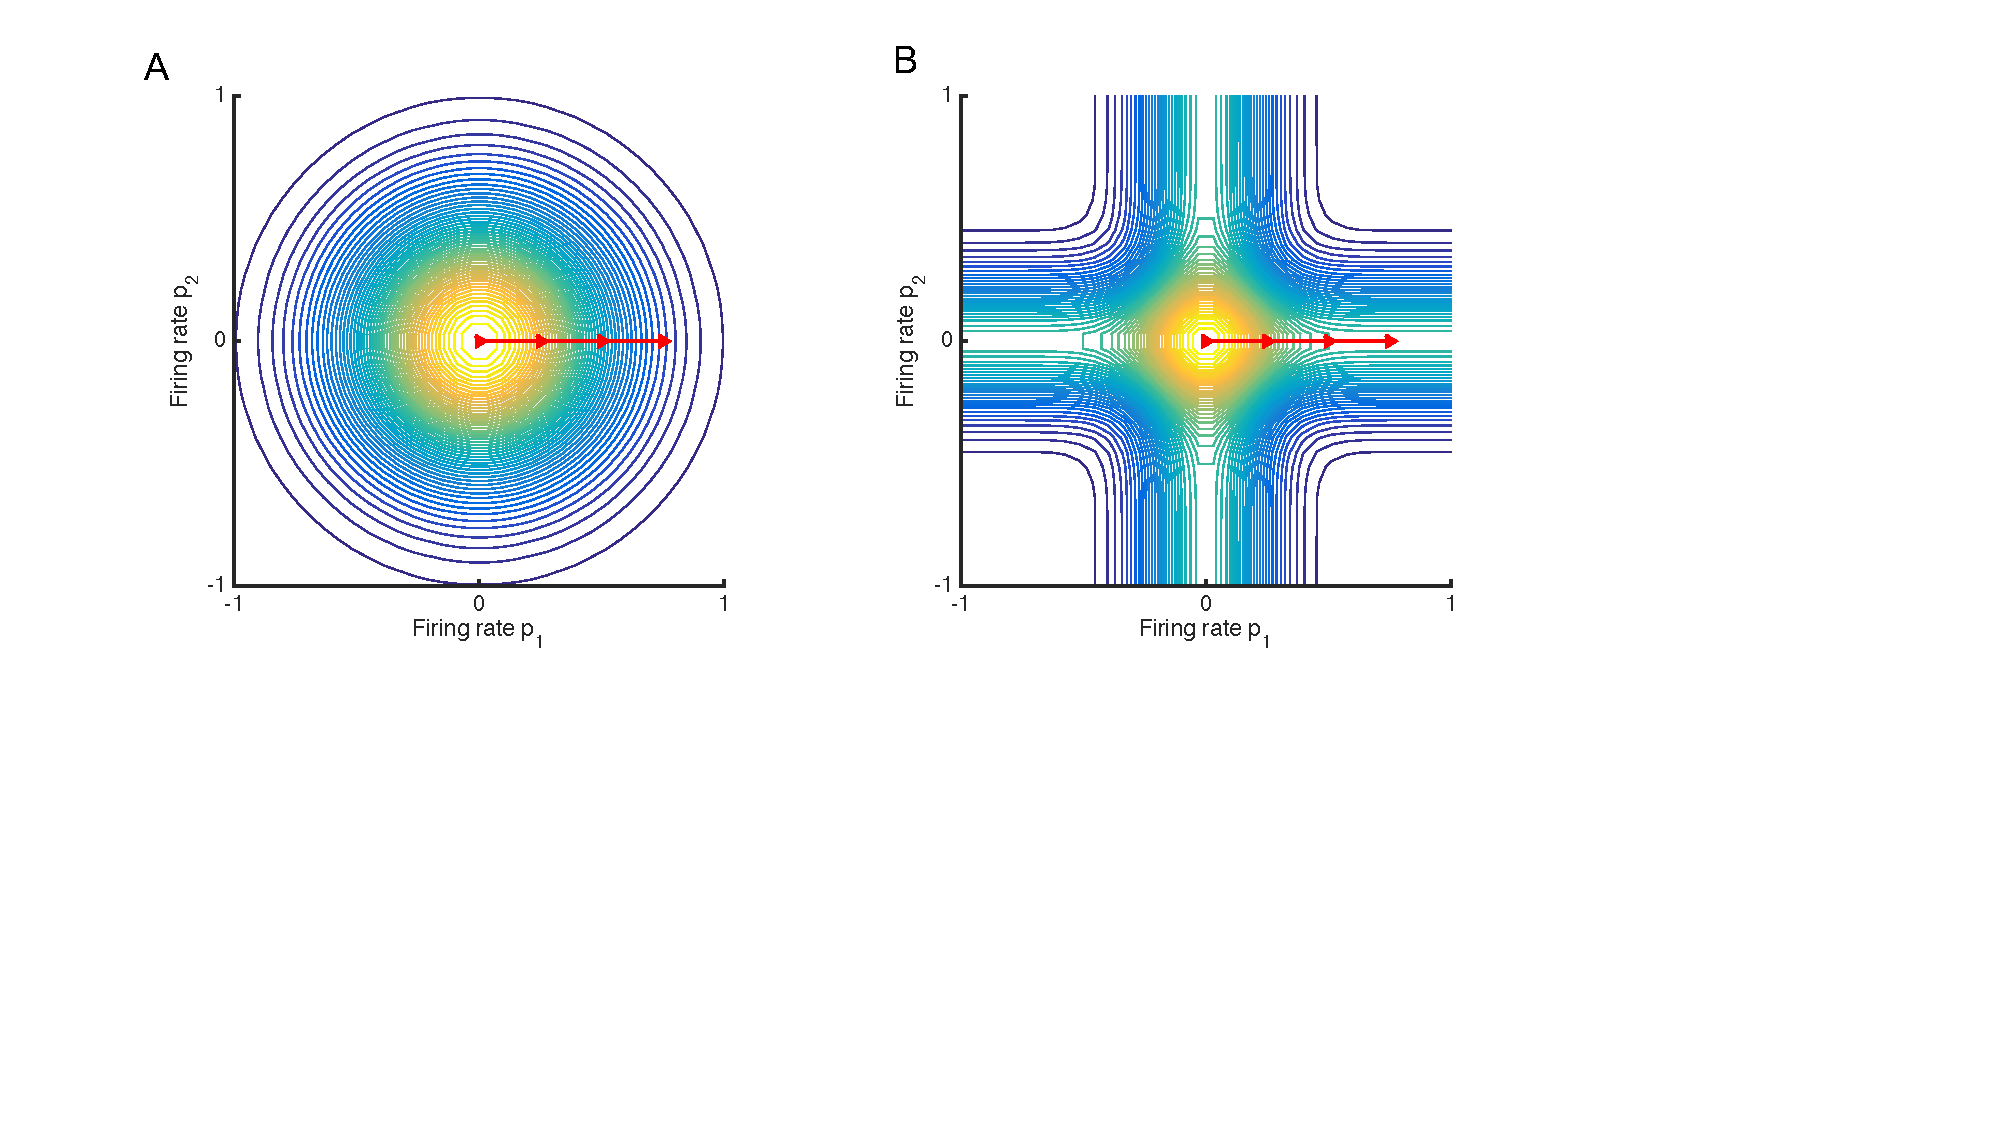
\includegraphics[width=\textwidth]{robustness_Fig1}
\caption[Schematic demonstrating the effect of kernel selection on the measure of similarity for 2-dimensional neural features]{Schematic demonstrating the effect of kernel selection on the measure of similarity for 2-dimensional neural features.  Since kernel similarity between two points only depends on their coordinate-wise differences, we let $p_1=(0,0)$ be a point at the origin and consider the kernel-determined similarity between $p_1$ and a second point $p_2=(x,y)$.  For each plot, the color at $(x,y)$ represents the measure of similarity according to the selected kernel $K_{\tilde\theta}(p_1,p_2)$.  Traveling along the red line illustrates the effect of increasing the difference in measurements for a single neuron. For the RBF kernel (A), moving along the arrow results in the kernel becoming arbitrarily small. By contrast, the MK kernel (B) never falls below 1/2 of the value at the origin as it moves along the arrow. For 40 dimensions, the MK kernel would never fall below 39/40 of its maximal value. Hence, when the RBF kernel is used for closed-loop decoding, nonstationarities from a single neural feature would result in no similarity between the current neural feature and any of the training data. By contrast, the MK kernel will remain relatively unaffected by even a drastic change in a single neuron, and continue to effectively use the information from the remaining neurons.}
\label{fig:kernel_illustration}
\end{figure}

\subsection{Training Set Sparsification for Robustness}

Training data was gathered during a standard radial center-out task during which the user attempted to move the cursor to one of eight equally-spaced targets arranged on a circle.  We took the (neural,velocity)-pairs and averaged the neural data over each of the eight targets.  The training set used for Gaussian process prediction consisted of these eight (average neural, velocity)-pairs.  Besides making prediction much faster, we found that using this sparsified training set additionally increased decoder robustness (see Results, cf. ~\cite{Sne05}).  

\section{Experimental Methods} \index{neural filtering!in humans|(}

\subsection{Permissions}

The Institutional Review Boards of Brown University, Partners Health/Massachusetts General Hospital and the Providence VA Medical Center, as well as The US Food and Drug Administration granted permission for this study (Investigational Device Exemption). The participants for this study were enrolled in a pilot clinical trial of the BrainGate Neural Interface System\footnote{ClinicalTrials.gov Identifier: NCT00912041. Caution: Investigational device. Limited by federal law to investigational use.}.

\subsection{Participant}

At the time of the study, T10 was a 35 year-old man with C4 AIS-A spinal cord injury. He underwent surgical placement of two 96-channel intracortical silicon microelectrode arrays \cite{Maynard1997} as previously described \cite{Simeral2011, Kim2008}. Electrodes were placed into the dominant precentral gyrus and dominant caudal middle frontal gyrus. Closed-loop recording data were used from trial (post-implant) days: 259, 265, 272, and 300. 

\subsection{Signal acquisition}

Raw neural signals for each electrode were sampled at 30kHz using the NeuroPort System (Blackrock Microsystems, Salt Lake City, UT) and then processed using the xPC target real-time operating system (Mathworks, Natick, MA). Raw signals were downsampled to 15kHz for decoding, and then de-noised by subtracting an instantaneous common average reference \cite{Jarosiewicz2015, Gilja2015} using 40 of the 96 channels on each array with the lowest root-mean-square value. The de-noised signals were band-pass filtered between 250 Hz and 5000 Hz using an 8th order non-causal Butterworth filter \cite{Masse2015}. Spike events were triggered by crossing a threshold set at $3.5\times$ the root-mean-square amplitude of each channel, as determined by data from a one-minute reference block at the start of each research session. The following neural features were extracted: (1) the rate of threshold crossings (not spike sorted) on each channel, and (2) the total power in the band-pass filtered signal \cite{Jarosiewicz2013, Jarosiewicz2015, Bacher2015, Brandman2018}.  A total of M=40 features were selected.  Neural features were binned in 20ms non-overlapping increments.

\subsection{Decoder calibration}

Task cueing was performed using custom built software running Matlab (Natick, MA). The participants used standard LCD monitors placed at 55-60 cm, at a comfortable angle and orientation. T10 engaged in the Radial-8 Task as previously described \cite{Jarosiewicz2013, Jarosiewicz2015, Bacher2015, Brandman2018}. Briefly, targets (size = 2.4 cm, visual angle = $2.5^\circ$) were presented sequentially in a pseudo-random order, alternating between one of eight radially distributed targets and a center target (radial target distance from center = 12.1 cm, visual angle = $12.6^\circ$). Successful target acquisition required the user to place the cursor (size = 1.5cm, visual angle = $1.6^\circ$) within the target's diameter for 300ms, before a pre-determined timeout (5 seconds). Target timeouts resulted in the cursor moving directly to the intended target, with immediate presentation of the next target. 

Each calibration block lasted 3 minutes. During calibration, decoder parameters were updated every 2-5 seconds as previously described \cite{Brandman2018}. During the initial stages of calibration, we assisted cursor performance by attenuating the component of the decoded velocity perpendicular to the target \cite{Jarosiewicz2013, Velliste2008}. This automated assistance was gradually decreased, until it was removed 100-130 seconds after the start of calibration. The coefficients for the MK-DKF decoder were computed using the calibration block used for the Kalman decoder. 

\subsection{Noise Injection Experiment} \index{Discriminative Kalman Filter!online human neural decoding experiment}

Once the decoder was calibrated, we sought to investigate the impact of nonstationarities to the MK-DKF and Kalman decoders. Our approach was to have T10 perform the Radial-8 Task, while randomly ``injecting noise'' to a single feature and also randomly selecting the decoder currently being used. 

Each trial ended after either (1) the target was acquired by having the cursor hold within the target for 300ms, or (2) a 5 second timeout. At the start of every noise injection trial, the cursor was (1) re-centered over the previously presented target, and (2) the velocity was reset to zero (this ensured that any potential impact of cursor's behavior from the previous trial was removed). We performed block randomization of the six experimental conditions: combining one of two decoders (Kalman and MK-DKF) with one of three noise levels (no noise, 1 z-score, 5 z-scores). Both the researchers and T10 were blinded to which decoder/noise combination was currently being used. To simulate noise, we provided a z-score offset to the channel with the highest signal to noise ratio \cite{Malik2015}, based on the value computed from the calibration block. We standardized the 40 features and the noise-injected feature for both the MK-DKF and Kalman decoders. Experiments were performed in 4 minute blocks. 

In order to ensure that T10 was blinded to the decoder and noise combination, we ensured that the kinematic ``feel'' of the decoders were similar. That is, we sought to match the mean speed, smoothing, and innovation terms for the two decoders, since these parameters are known to impact decoding quality \cite{Willett2017}. For the Radial-8 noise-injection experiment, we matched kinematic parameters in two ways. First, we set the $A$ and $\Gamma$ of \eqref{e:DKF} to match the Kalman values. Second, to ensure that both decoders moved at the same speed, we first computed the mean speed values for $K\zeta$ in the training block. Next, we computed the mean speed value of $f(x_t)$, and then linearly scaled $f(x_t)$ to match the mean $K\zeta$ value. 

Hence, in performing head-to-head comparisons we opted to match the kinematics of the MK-DKF decoder to the Kalman. We note that it is \emph{very likely} that we were negatively impacting the MK-DKF decoder performance by doing so, since the parameters used were likely sub-optimal compared to those that would have been computed. 

%%%%%%%%%%%%%%%%%%%%%%%%%%%%%%%%%%%%%%%%%%%%%%%%%
\begin{figure}[h]
\begin{minipage}[c]{.33\textwidth}
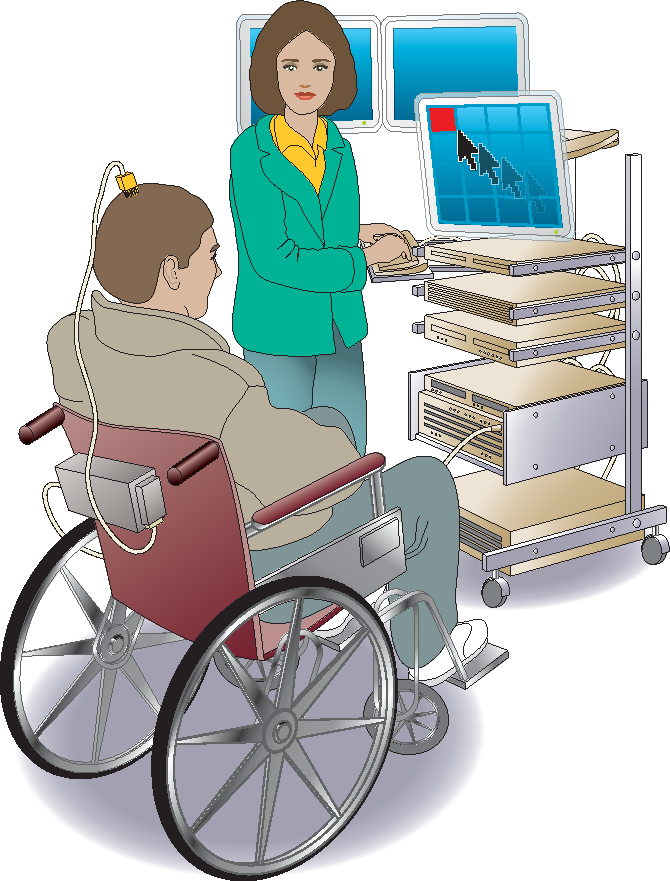
\includegraphics[width=\linewidth]{bg_setup_diagram}
\end{minipage}
\hfill
\begin{minipage}[c]{.66\textwidth}
\caption[The BrainGate cart setup]{All equipment necessary for decoding is based on a cart that can be stored in the participant's home.}
\end{minipage}
\end{figure}

\subsection{Performance measurement}

We quantified performance using a Grid Task after locking decoder parameters \cite{Brandman2018, Pandarinath2017, Nuyujukian2015}. This task consisted of a grid of 36 square targets arranged in a square grid, where the length of one side of square grid was 24.2 cm (visual angle = $24.8^{\circ}$). One of 36 targets was presented at a time in a pseudo-random order. Targets were acquired when the cursor was within the area of the square for 1 second. Incorrect selections occurred if the cursor dwelled on a non-target square for an entire hold period. Each comparison block was 3 minutes in length. 

We measured the achieved bit rate (BR), which measures the effective throughput of the system \cite{Nuyujukian2015}:

\begin{equation*}
\text{BR} = \frac{\log_2(N - 1) ~ \max(S_c - S_i, 0)}{t}
\end{equation*}
where $N$ is the number of possible selections, $S_c$ and $S_i$ are the number of correctly and incorrectly selected targets, respectively, and $t$ is the elapsed time within the block. 
\index{neural filtering!in humans|)}

\subsection{Offline analysis}

We retrospectively analyzed data collected from previous research sessions. We restricted our analysis to sessions where T10 moved a computer cursor using motor imagery. He acquired targets using the Radial-8 task, the Grid Task, or free typing tasks \cite{Jarosiewicz2015}. 

\subsubsection{Injecting noise for the MK-DKF and Kalman decoders}

To investigate the impact of noise on decoder performance, we performed offline simulations of both the Kalman and MK-DKF decoders. We computed the angular error between the predicted decoder value without filtering (i.e. the $Kz$  term and the $f(x_t)$ terms of the Kalman and MK decoders, respectively) and the label modeled as the vector from cursor to target \cite{Simeral2011, Brandman2018}. Data from a single research session were concatenated together. A decoder was trained using half of the data available for a session without replacement, and then used to predict the mean angular error for the other half of the dataset. Decoder predictions were bootstrapped 100 times.  
 
\subsubsection{Offline assessment of noise}

As part of feature pre-processing for closed-loop decoding with the Kalman filter, we performed z-score normalization of the neural features. The incoming features are normalized using the mean and the standard deviation of the previous block's worth of data; this has the effect of increasing cursor control quality by attempting to address signal nonstationarities \cite{Jarosiewicz2015}. Our standard practice is to use a subset of the channels, selected according to a signal to noise ratio \cite{Malik2015}. Our standard practice is to recalibrate the Kalman decoder at user-defined intervals. That is, we recompute the $K$ Kalman between blocks when the researcher is setting up the next experiment, or the user is taking a break \cite{Jarosiewicz2015}.

For each session, we incrementally calibrated Kalman decoders in chronological order. We then computed the number of times a feature exceeded a z-score offset in the next block. For instance, to compute the number of noise events at 2 z-scores for Trial Day 295 Block 5, we computed the z-score mean and standard deviations based on data for Blocks 1-4, and then counted the number of 20ms blocks with deviations more than 2 z-scores away from the mean for each feature.

\section{Results}

\subsection{Quantifying the effect of noise on closed-loop neural decoding}

We investigated the impact of noise injection for both the Kalman and MK-DKF decoders by performing offline simulations of previously collected data. There were a total of 124 research sessions recorded from participant T10. We identified 97 sessions and a total of 48.2 hours of closed-loop neural control of a computer cursor, during which many variations of neural decoders had been explored. For each of the 97 sessions, we bootstrapped the data 100 times into non-overlapping training and testing sets (50/50 splits), and then used the training dataset to compute the coefficients for both the Kalman and MK-DKF decoders. We measured decoder performance using the predicted angular error between the simulated decoded direction and the known vector from cursor to target (see methods). 

\begin{figure}[h]
\centering
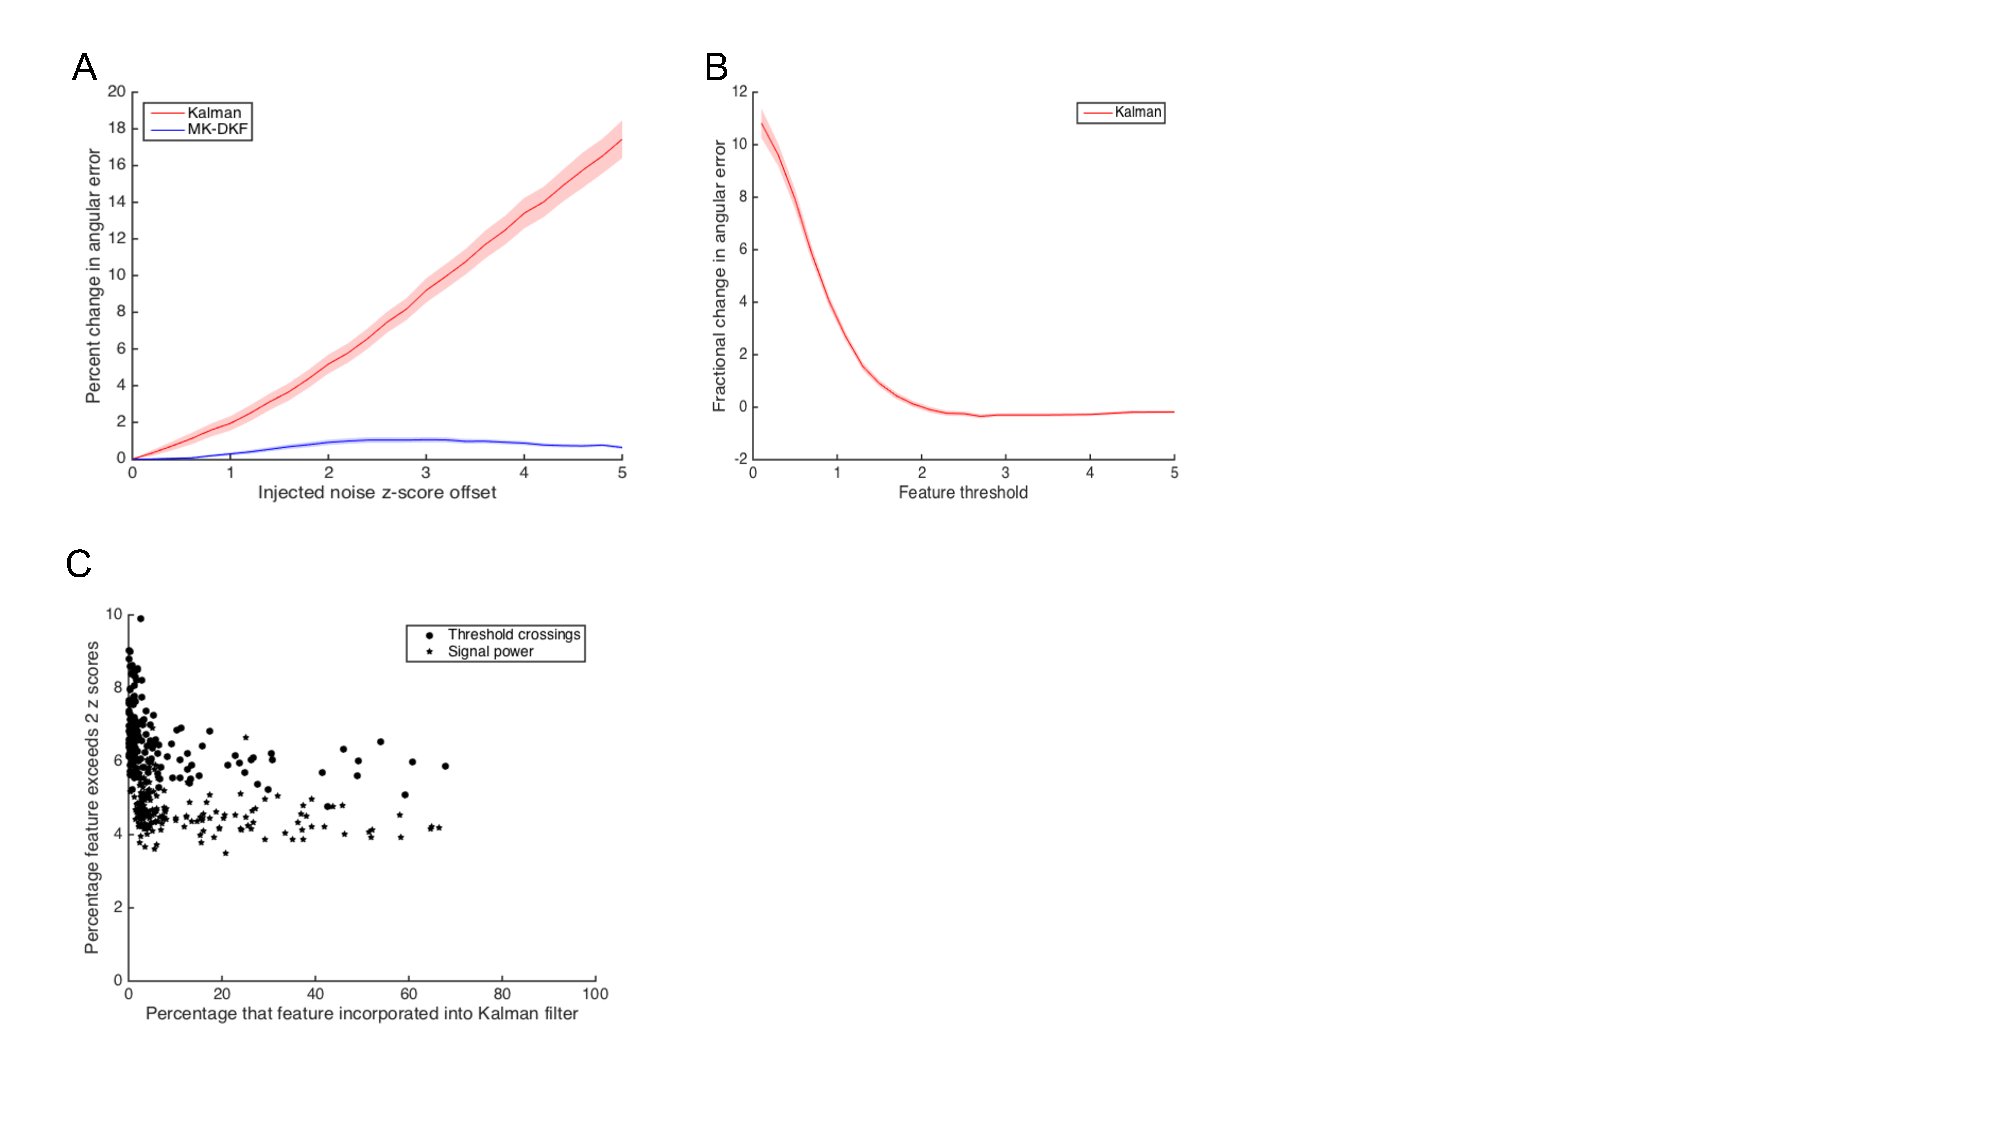
\includegraphics[width=\textwidth]{robustness_Fig2}
\caption[Offline performance comparison of nonstationary noise injection on Kalman and MK-DKF decoders]{A: Change in angular error as a function of z-score offset for both the Kalman and MK-DKF decoders. We identified 96 research sessions where T10 performed closed-loop neural control. For each session, we performed a 50/50 split, using the training data to compute the coefficients for the Kalman and MK-DKF decoders, and then predicting the angular error on the testing data. Next, we added a z-score offset to a single channel (standardized for each decoder). The shaded areas represent the standard error of measurement for each decoder. B: Change in angular error as a function of feature thresholding. During the bootstrapping procedure, we saturated features for both the training and testing datasets, and computed the change in angular error compared to no saturation. The shaded area represents the standard error of measurement. C: Examining the frequency of noise events. For each of the bootstrapped simulations, we counted the frequency at which each feature was incorporated into the decoder ($m = 40$), as well as the frequency at which the feature was observed to deviate by more than 2 z-scores.}
\label{fig:Fig2}
\end{figure}

Our implementation of the Kalman decoder for closed-loop neural control \cite{Jarosiewicz2015, Bacher2015, Brandman2018} uses a measure of signal-to-noise to sub-select 40 of the 384 features to be used in closed-loop decoding \cite{Malik2015}. We added noise to the single feature with the highest signal to noise ratio in the testing dataset (Fig 2A). With the Kalman decoder, we found a nearly linear relationship between the amount of injected noise and the percent change in angular error ($R^2 = 0.994, p < 10^{-24}$). We then repeated this experiment using the same features for both calibration and noise injection with the MK-DKF decoder. We found that noise injection had only minimal changes to the MK-DKF performance despite large noise injection values. 

Given the detrimental effect of z-score offsets on decoding performance, a straightforward solution would be to simply ``saturate'' the features used for decoding. That is, all values greater than a saturation value (e.g. 2 z-scores) would be set to the saturation value. We computed the change in angular error as a function of feature saturation threshold (Fig 2B). We found that the angular error decreased as saturation levels increased, reaching the base performance at 2 z-scores. These results suggested that features could be saturated at 2 z-scores without negatively impacting decoding performance. 

Next, we quantified the frequency at which 2 z-score noise events occurred. Across all features, the 2 z-score deviations occurred 5.6\% $\pm 1.2$ (std) of observed 20ms bins (Fig 2C). Importantly, the same features that had large noise events were those that were highly informative and incorporated into the Kalman filter according to the feature's SNR \cite{Jarosiewicz2015, Bacher2015, Brandman2018}. Since real-time neural decoding is commonly performed in 20ms bins, these results suggest that apparent noise events are observed roughly 3 times per second with our current clinical research-grade neural recording setup. 

Taken together, these results suggest that: (1) the Kalman decoder is highly sensitive to z-score offsets, even arising from a single feature; (2) z-score offsets that degrade decoding performance for the Kalman occur approximately 3 times per second; (3) principled thresholding of features will alleviate some, but not all, of the effects of z-score offsets. These results also suggest that the MK-DKF is relatively insensitive to z-score offsets for single features. 

\subsection{Online analysis: Closed loop assessment of both the Kalman and MK-DKF decoders} \index{neural filtering!in humans}

We characterized the effect that noise events had on closed-loop neural decoding with T10 (Fig 3A, Supplementary Movie 1). At the start of the research session, we first calibrated both the Kalman and MK-DKF decoders, and then matched their kinematics coefficients and the subset of features used for decoding. Next, we performed a double-blinded randomization procedure where both the decoder and the amount of noise injected were randomly selected every two targets. Neither T10 nor the researchers were aware of the current decoder/noise combination. Noise was injected by offsetting the z-score of a single feature, standardized for both decoders (see Methods).

\begin{figure}[h]
\centering
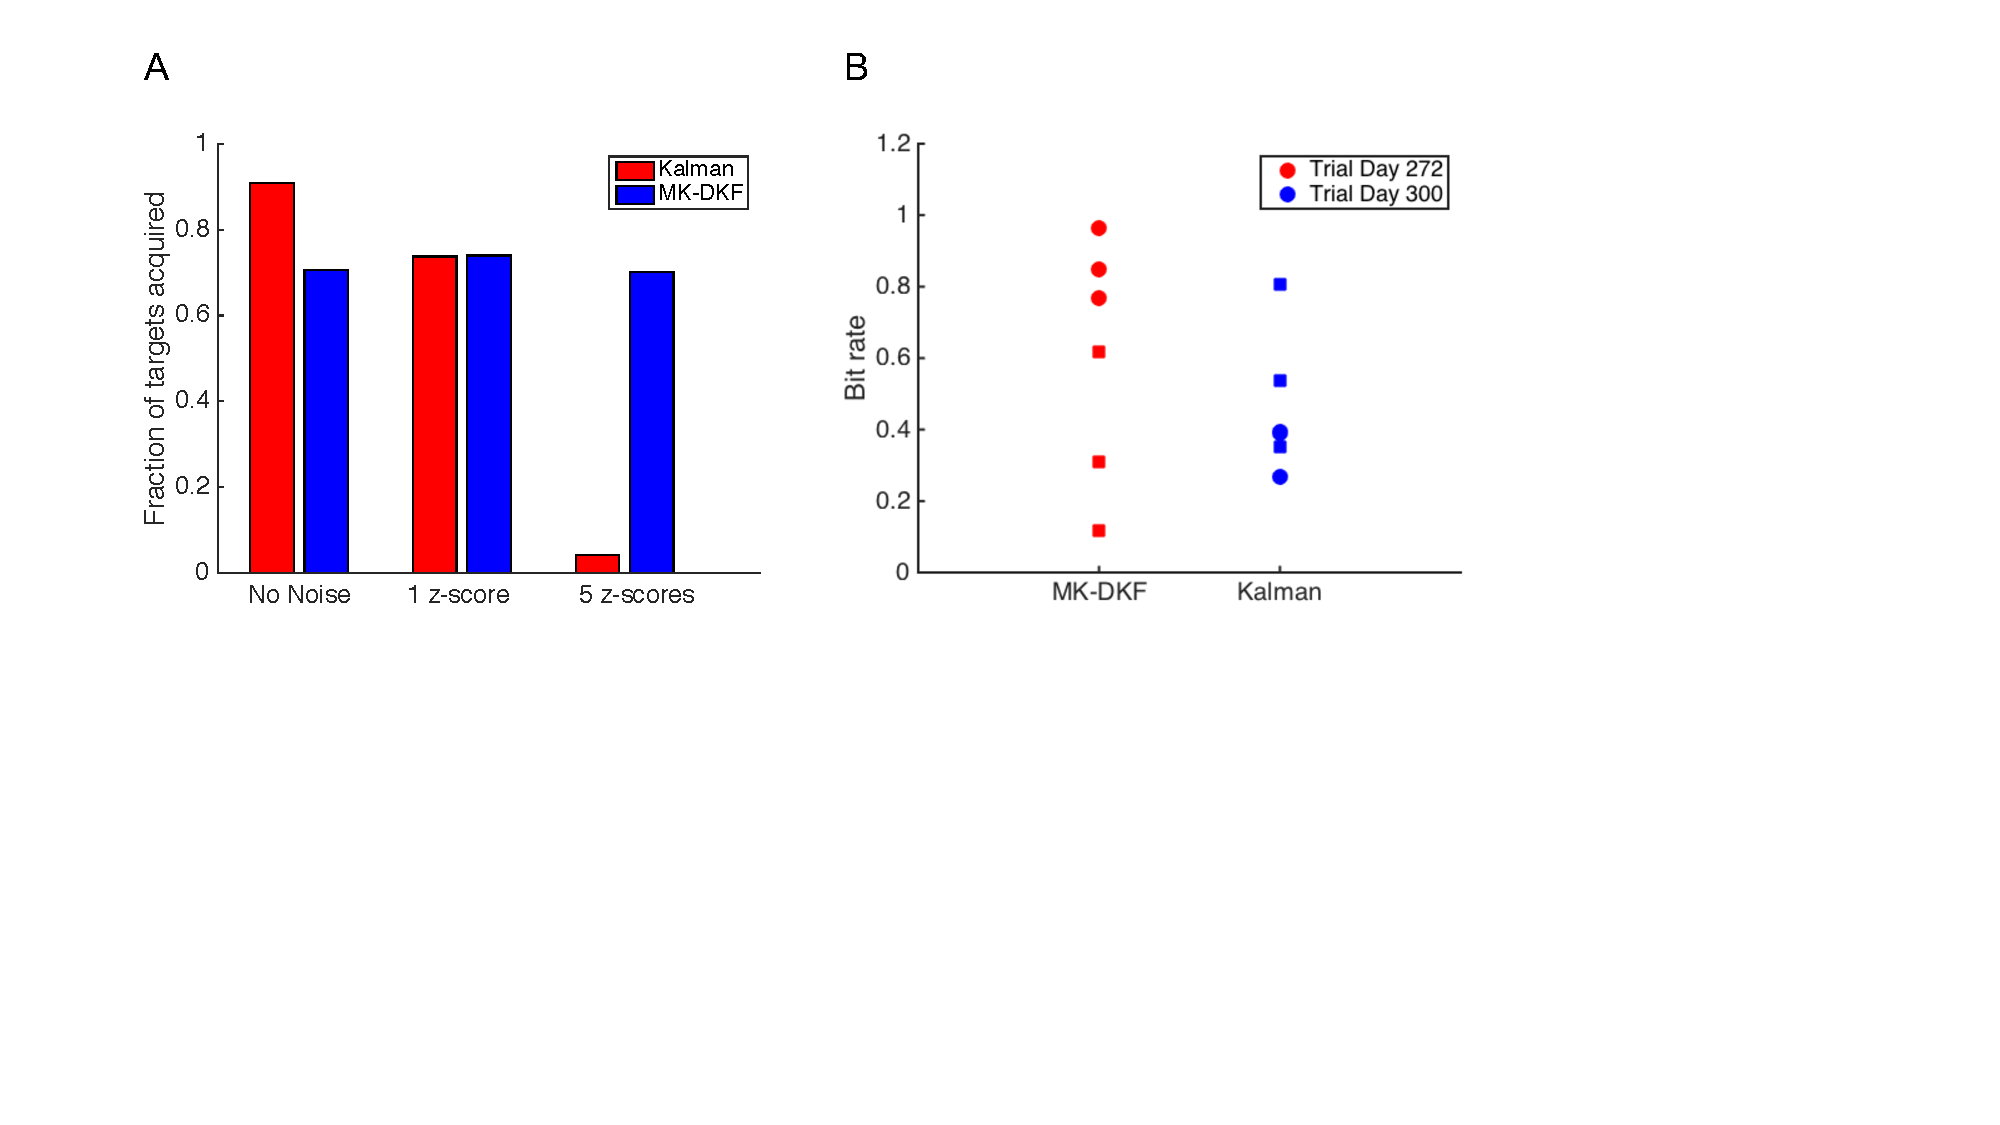
\includegraphics[width=\textwidth]{robustness_Fig3}
\caption[Online performance comparison of nonstationary noise injection on Kalman and MK-DKF decoders]{A: Targets acquired during closed-loop Radial-8 control by T10. On research Days 259, 265, 272, and 300, T10 acquired targets in a Radial-8 task wherein the decoder (Kalman and MK-DKF) and the amount of noise (no noise, 1 z-score, 5 z-scores) were randomly selected. There was no statistically significant difference in performance across the noise injection trials for the MK-DKF decoder ($\chi^2, p = 0.81$) There was a statistically significant difference across conditions for the Kalman decoder ($\chi^2, p < 10^{-37}$). These conditions were performed with the kinematic parameters of the MK-DKF matched to the Kalman decoder. B: Performance of both the MK-DKF and Kalman decoders with optimal kinematic parameters. There was no statistically significant difference in bit rate between the two decoders (Trial Days 272 and 300, Wilcoxon rank-sum test p = 0.48).}
\label{fig:Fig3}
\end{figure}

T10 was presented with a total of 596 targets in a center-out task over three research sessions (Trial Days 259, 265, and 272). For the Kalman decoder, there was a statistically significant dose dependent response between the amount of injected noise (no noise, 1 z-score offset, and 5 z-score offsets) and the fraction of targets acquired within a 5 second timeout ($\chi^2, p < 10^{-37}$). By contrast, there found no statistically significant difference between the three noise conditions with the MK-DKF decoder ($\chi^2, p = 0.81$). 

We note that in this comparison, the fraction of targets acquired by the MK-DKF decoder was inferior to that of the Kalman decoder without injected noise. In order to have performed this comparison, we matched the kinematic coefficients of the MK-DKF to the Kalman decoder (see methods). This ensured that the ``feel'' of the decoders were indistinguishable, allowing us to perform the randomized experiment. However, in so doing, we were likely selecting sub-optimal kinematic coefficients for the decoder.

To quantify the performance of both decoders without injected noise and with optimal kinematic parameters, we calibrated the Kalman and MK-DKF decoders using their respective optimal kinematic coefficients. After decoder calibration, T10 acquired targets in the Grid Task, and the decoder being used was alternated every block (Fig 3B). We found there was no statistically significant difference in bit rate between the two decoders (Trial Days 272 and 300, Wilcoxon rank-sum test p = 0.48). 

\section{Discussion}

A new class of neural decoder based on Gaussian process regression was more resilient to noise than the traditionally used linear decoding strategy used for closed-loop neural control. When z-score offsets were added to single channels in the Kalman filter, the decoding performance degraded; this was not seen with the MK-DKF decoding approach. After optimizing the parameterizations of both decoders, the communication bit-rate was not statistically different. 

\subsection{Addressing nonstationarities in neural data} \index{neural filtering!nonstationarities} 

Robust and reliable control with an intracortical brain computer interface is predicated on the properties of the decoding algorithm selected to map high-dimensional neural features to low-dimensional commands used to control external effectors. End-effector control degrades without recalibration of decoder parameters \cite{Jarosiewicz2015, Perge2013}. To this end, multiple solutions have been proposed to recalibrate decoders based on closed-loop neural data during use, either when targets are known \cite{Hochberg2006, Kim2008, Hochberg2012, Jarosiewicz2013, Collinger2013, Wodlinger2015, Gilja2015, Orsborn2014, Shanechi2017, Dangi2011, Carmena2013} or retrospectively inferred \cite{Jarosiewicz2015}. Other approaches have investigated BCI decoder robustness using a wide variety of specific methods, including: adapting a discriminative Bayesian filter~\cite{Brandman2018}, refitting a Kalman filter~\cite{Gil12, Dan13}, Bayesian updating for an unscented Kalman filter~\cite{Li11}, reweighting a na\"ive Bayes classifier~\cite{Bis14}, retraining a kernelized ARMA model~\cite{Shp09}, and reinforcement learning~\cite{Mah13,Poh14}, among others.  

Rather than adapting the coefficients of the decoder given new closed-loop data, the goal of robust model selection is to design the decoder to be more resilient to nonstationarities. One previously described decoder achieved robustness with a multiplicative recursive neural network and augmenting the training data with perturbations that mimicked the desired nonstationities against which they wished to train ~\cite{Sus16}. For example, in order to train against dropping the $i$th neuron, exemplars were added to the training dataset where the $i$th neuron had been zeroed-out.  This technique of augmenting a training set with noisy data is well-established for increasing generalization performance in neural networks, and is commonly referred to as data augmentation~\cite{An96}.  It requires generating and training over new artificial data for each individual targeted nonstationarity for each feature.  Hence, exemplars generated to protect the decoder against dropping the $i$th feature do not protect against dropping the $j$th feature. 

While effective, there are limitations in applying data augmentation for closed-loop BCI systems for human users. First, one of the goals of pursuing iBCI research for people is to develop devices that are intuitive and easy to use, with minimal technician oversight, and requiring calibration. It would not be possible to apply a deep neural network with bagging technique in the case where the user is using the system with limited available data, such as using the system for the first time \cite{Brandman2018}. Second, the system requires significant computational resources. Bagging enlarges an already massive dataset by orders of magnitude, entailing a commensurate increase in training burden for the neural network. At least with today's available hardware and the requirement for local computation, the increase in computational resources would not be possible for portable iBCI systems to be used inside the homes of users.  

By contrast, the MK-DKF decoder did not require explicit training to acquire robustness. The robust kernel design was able to distinguish between signal and noise within three minutes of calibration.

\subsection{Growth directions for MK-DKF}

Our implementation of the MK-DKF decoder provides an exciting foundation from which to explore decoder robustness. For instance, our approach na\"ively provided a uniformly weighted linear addition of multiple kernels, thereby making the explicit assumption that each feature is equally important for decoding. One approach would be to incorporate techniques in kernel learning \cite{Gonen2011}. For instance, one could learn a convex sum of weights for the linear combination of kernels that ``align'' to a training kernel \cite{Cortes2012}. Alternatively, one could be explore alternative distance metrics. For instance, rather than using Euclidean distances between features, one could apply a spike-train distance metric \cite{Victor1997a}. This metric can be adapted as a valid kernel embedding function and used for decoding neural data \cite{Park2013, Brockmeier2014, Li2014}. It has also been shown to perform better than Euclidean distances when visualizing complex neuronal datasets \cite{Vargas-Irwin2015}.

\section{Conclusion}

In order for BCIs to succeed as an assistive technology, they will need to perform well over longer periods of time without user feedback or manual recalibration.  Incorporating a robust model allows a filter to anticipate nonstationarities and seamlessly adapt to them.  Here we present the first experimental evidence that a fixed, robust decoder can provide reliable and high quality neural cursor control in the presence of injected nonstationarities.

\section{Acknowledgements}

The authors would like to thank participant T10 and their family; B. Travers, and D. Rosler for administrative support; C. Grant for clinical assistance; and Prof. Arthur Gretton for discussions on kernel selection. This work was supported by the National Institutes of Health: National Institute on Deafness and Other Communication Disorders - NIDCD (R01DC009899), Rehabilitation Research and Development Service, Department of Veterans Affairs (B6453R and N9228C); National Science Foundation (DMS1309004), National Institute of Health (IDeA P20GM103645, R01MH102840); Massachusetts General Hospital (MGH) - Deane Institute for Integrated Research on Atrial Fibrillation and Stroke; Joseph Martin Prize for Basic Research; the Executive Committee on Research (ECOR) of Massachusetts General Hospital; Canadian Institute of Health Research (336092); Killam Trust Award Foundation; Brown Institute of Brain Science. The content of this paper is solely the responsibility of the authors and does not necessarily represent the official views of the National Institutes of Health, the Department of Veterans Affairs or the United States Government.

